\documentclass[11pt]{article}
\usepackage[a4paper,margin=2.2cm]{geometry}
\usepackage{graphicx}
\usepackage{booktabs}
\usepackage{parskip}
\usepackage{caption}

\setlength{\parindent}{0pt}
\pagestyle{empty}

\begin{document}

{\Large\bfseries C51 (Categorical DQN) on Pong: progress report}\\[2pt]
Group 27 \textbullet{} Topic 27 (C51, IQN, Rainbow, IMPALA) \textbullet{} JAXAtari baselines

\vspace{6pt}\hrule\vspace{8pt}

C51 is implemented in JAX/Flax as a single self-contained file supporting both
observation modes (pixel with a CNN, object-centric with an MLP).
\textbf{Both modes solve Pong.}

\vspace{4pt}
\begin{center}
\begin{tabular}{@{}llcc@{}}
\toprule
Mode & Network & Final return (10M) & Reference \\
\midrule
Pixel           & CNN & $\mathbf{+20.6}$ & CleanRL C51 $\approx +20$ \\
Object-centric  & MLP & $\mathbf{+19.0}$ & no OC reference \\
\bottomrule
\end{tabular}
\end{center}

\begin{figure}[h]
\centering
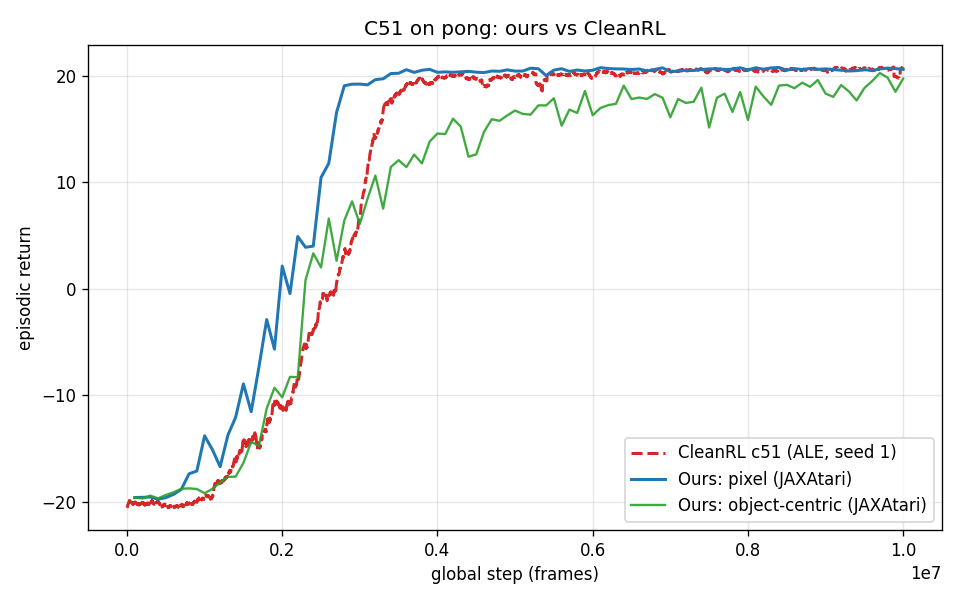
\includegraphics[width=0.72\linewidth]{c51_vs_cleanrl.png}
\caption*{\small Episodic return on Pong (10M frames): our pixel and object-centric runs
vs the CleanRL \texttt{c51\_atari\_jax} reference curve (ALE). Our pixel matches CleanRL;
object-centric learns slower but reaches $+19$. Both runs use CleanRL's exact
update-to-data ratio (one gradient update per 4 frames).}
\end{figure}

\textbf{Object-centric finding.}
Object-centric observations needed normalization (the raw pixel-coordinate features were
saturating the MLP); adding \texttt{NormalizeObservationWrapper} plus a $512\times512$ MLP
fixed it. Same fix will apply to IQN, Rainbow and IMPALA.

\vspace{6pt}
\textbf{Questions for feedback}
\begin{enumerate}\itemsep2pt
  \item Pixel matches the reference. Enough to call C51 pixel done, or do you want
        multi-seed variance bands?
  \item OC uses \texttt{Normalize} $+ 512\times512$ instead of
        CleanRL's CartPole MLP. OK to keep?
\end{enumerate}

\newpage

{\large\bfseries Training metrics: ours vs CleanRL (10M)}

\vspace{8pt}
\begin{figure}[h]
\centering
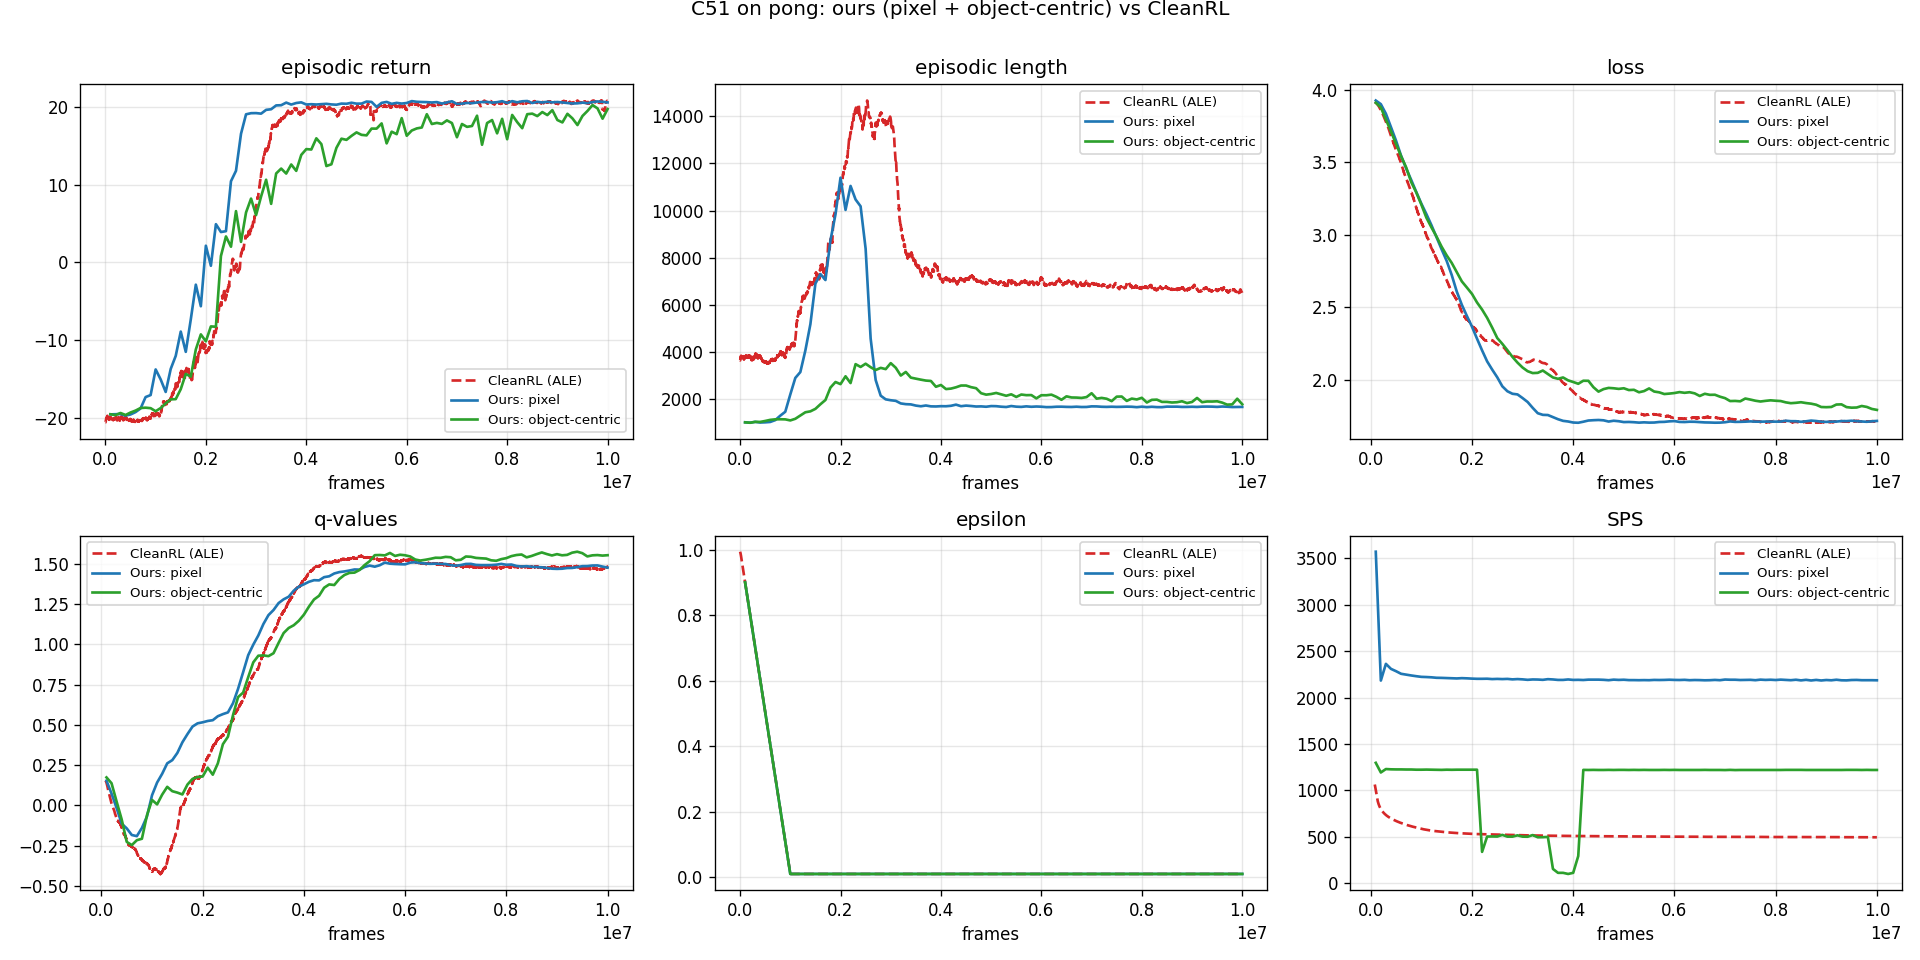
\includegraphics[width=\linewidth]{c51_all_vs_cleanrl_metrics.png}
\caption*{\small Six metrics, three curves each: CleanRL \texttt{c51\_atari\_jax} (ALE),
our pixel, and our object-centric. Loss, epsilon and q-values track CleanRL closely; SPS
is higher for ours even at 8 envs (JAXAtari runs the env on GPU). Episode length is counted
differently by JAXAtari than ALE.}
\end{figure}

\end{document}
